%%%%%%%%%%%%%%%%%%%%%%%%%%%%%%%%%%%%%%%%%
% Short Sectioned Assignment
% LaTeX Template
% Version 1.0 (5/5/12)
%
% This template has been downloaded from:
% http://www.LaTeXTemplates.com
%
% Original author:
% Frits Wenneker (http://www.howtotex.com)
%
% License:
% CC BY-NC-SA 3.0 (http://creativecommons.org/licenses/by-nc-sa/3.0/)
%
%%%%%%%%%%%%%%%%%%%%%%%%%%%%%%%%%%%%%%%%%

%----------------------------------------------------------------------------------------
%	PACKAGES AND OTHER DOCUMENT CONFIGURATIONS
%----------------------------------------------------------------------------------------

\documentclass[paper=a4, fontsize=11pt]{scrartcl} % A4 paper and 11pt font size

\usepackage[T1]{fontenc} % Use 8-bit encoding that has 256 glyphs
%\usepackage{fourier} % Use the Adobe Utopia font for the document - comment this line to return to the LaTeX default
\usepackage[english]{babel} % English language/hyphenation
\usepackage{amsmath,amsfonts,amsthm} % Math packages

\usepackage{sectsty} % Allows customizing section commands
%\allsectionsfont{\centering \normalfont\scshape} % Make all sections centered, the default font and small caps
\allsectionsfont{\centering}

\usepackage{fancyhdr} % Custom headers and footers
\pagestyle{fancyplain} % Makes all pages in the document conform to the custom headers and footers
\fancyhead{} % No page header - if you want one, create it in the same way as the footers below
\fancyfoot[L]{} % Empty left footer
\fancyfoot[C]{} % Empty center footer
\fancyfoot[R]{\thepage} % Page numbering for right footer
\renewcommand{\headrulewidth}{0pt} % Remove header underlines
\renewcommand{\footrulewidth}{0pt} % Remove footer underlines
\setlength{\headheight}{13.6pt} % Customize the height of the header

%\numberwithin{equation}{section} % Number equations within sections (i.e. 1.1, 1.2, 2.1, 2.2 instead of 1, 2, 3, 4)
%\numberwithin{figure}{section} % Number figures within sections (i.e. 1.1, 1.2, 2.1, 2.2 instead of 1, 2, 3, 4)
%\numberwithin{table}{section} % Number tables within sections (i.e. 1.1, 1.2, 2.1, 2.2 instead of 1, 2, 3, 4)

\setlength\parindent{0pt} % Removes all indentation from paragraphs - comment this line for an assignment with lots of text

\usepackage{caption}

\usepackage{algorithm}
\usepackage[noend]{algorithmic}

%\floatname{algorithm}{Procedure}
\renewcommand{\algorithmicrequire}{\textbf{Input:}}
\renewcommand{\algorithmicensure}{\textbf{Output:}}

\newtheorem{mydef}{Definition}
\theoremstyle{plain}
\newtheorem{lemma}{Lemma}


\usepackage{graphicx}
\graphicspath{{../images/}}



%----------------------------------------------------------------------------------------
%	TITLE SECTION
%----------------------------------------------------------------------------------------

\newcommand{\horrule}[1]{\rule{\linewidth}{#1}} % Create horizontal rule command with 1 argument of height

\title{	
\normalfont \normalsize 
\textsc{UPC - Discrete and algorithmic geometry} \\ [25pt] % Your university, school and/or department name(s)
\horrule{0.5pt} \\[0.4cm] % Thin top horizontal rule
\huge Problem sheet 1  \\ % The assignment title
\horrule{2pt} \\[0.5cm] % Thick bottom horizontal rule
}

\author{Simon Van den Eynde} % Your name

\date{\normalsize\today} % Today's date or a custom date

\begin{document}

\maketitle % Print the title

%----------------------------------------------------------------------------------------
%	Problem 9
%----------------------------------------------------------------------------------------
\section{a}
$P+Q$ is convex if all line segments joining two points of the polytope is contained in the polytope. And we will prove that it happens only if $P$ and $Q$ are convex.

$$P+Q\subset \mathbb{R}^d \quad convex \Longleftrightarrow \forall s_1,s_2 \in P+Q \quad s_1 s_2 \subset P+Q$$

Take two points $s_1,s_2\in P+Q$. Then, $\exists p_1,p_2 \!\! \in \!\! P$, $\exists q_1,q_2 \!\! \in \!\! Q$ such that $s_1 = p_1 + q_1$ and $s_2= p_2 + q_2$.\\

Let $r\in s_1 s_2$ be any point of the segment. Then, $\exists \lambda \in [0,1]$ such that $r = \lambda s_1 + \left( 1 - \lambda \right) s_2$.\\

Expanding it:

$r = \lambda s_1 + \left( 1 - \lambda \right) s_2 = \lambda \left(p_1 + q_1 \right) + \left( 1 - \lambda \right) \left( p_2 + q_2 \right) = \lambda p_1 + \left( 1 - \lambda \right) p_2 + \lambda q_1 + \left( 1 - \lambda \right) q_2$\\

If $P$ and $Q$ are convex, then $p_1p_2 \subset P$ and $q_1q_2 \subset Q$, so $\exists p \!\! \in \!\! P$ s.t. $p = \lambda p_1 + \left( 1 - \lambda \right) p_2$ and $\exists q \!\! \in \!\! Q$ s.t. $q = \lambda q_1 + \left( 1 - \lambda \right) q_2$.\\

So $r = p + q \in P+Q \quad \forall r \in s_1s_2 \Longrightarrow s_1s_2 \subset P+Q$ for any $s_1,s_2 \in P+Q$

Finally, $P+Q$ is convex if $P$ and $Q$ is convex.\\

Translating $P$ and $Q$ in $\mathbb{R}^d$ is the same as summing a single point to each. Let $p',q' \in \mathbb{R}^d$ be the points that represent the translation of $P$ and $Q$. Then $(P+p') + (Q+q') = \{p + q : p\in P + p',\,q\in Q + q'\} = \{p + p' + q + q' : p\in P,\,q\in Q\} = (P+Q)+p'+q'$

So $P+Q$ translates with the composition of the translations of $P$ and $Q$.

\section{b}
\begin{lemma}
New($fg$)=New($f$)+New($g$) for polynomials $f(x)=\sum_{i=1}^{m}{c_{i}x_{1}^{a_{i1}}x_{2}^{a_{i2}}\ldots x_{d}^{a_{id}}}$ and $g(x)=\sum_{i=1}^{p}{d_{i}x_{1}^{b_{i1}}x_{2}^{b_{i2}}\ldots x_{d}^{b_{id}}}$
\end{lemma}
\begin{proof}
We note that $fg(x)=\sum_{i=1}^{m}\sum_{j=1}^{p}{c_{i}d_{j}x_{1}^{a_{i1}+b_{j1}}x_{2}^{a_{i2}+b_{j2}}\ldots x_{n}^{a_{id}+b_{jd}}}$.\\
So New($fg$) is the convex hull of points of the form $(a_{i1}+b_{j1},a_{i2}+b_{j2},\ldots,a_{id}+b_{jd})$.
These points are thus of the form $p$+$q$ with $p\in$ New($f$) and $q\in$ New($g$), so New($fg)\subset$ New($f$)+New($g$).\\

Now choose a vertex $v\in$ New($f) +$ New($g$). Then $v=(a_{i1},a_{i2},\ldots,a_{id}) + (b_{j1},b_{j2},\ldots,b_{jd})$ for some $i$ and $j$. Then also $c_{i}\neq 0 \neq d_{j}$ and therefore $c_{i}d_{j}\neq0$, so $v\in$ New($fg$).
\end{proof}

\section{c}
From the polynomials we can easily derive the points we get to construct the convex hull. For $f$ we find $(0,0),(0,1),(1,1),(1,0)$ and for $g:(0,0),(2,1),(1,2)$.\\
I drew a picture in Figure~\ref{fig:cl}. From this picture we can derive that the area($P)= 1$, the area$(Q) = 4-2-\frac{1}{2} = 1.5$ (we distract from the 2-by-2 square two half 1-by-2 rectangles and half a unit square) and area$(P+Q) = 9 - 2 -\frac{1}{2} = 6.5$ (we distract from the 3-by-3 square two half 1-by-2 rectangles and half a unit square).
So $M(P,Q) = 6.5-1-1.5 = 4$.

\begin{figure}[htbp]
   \centering
   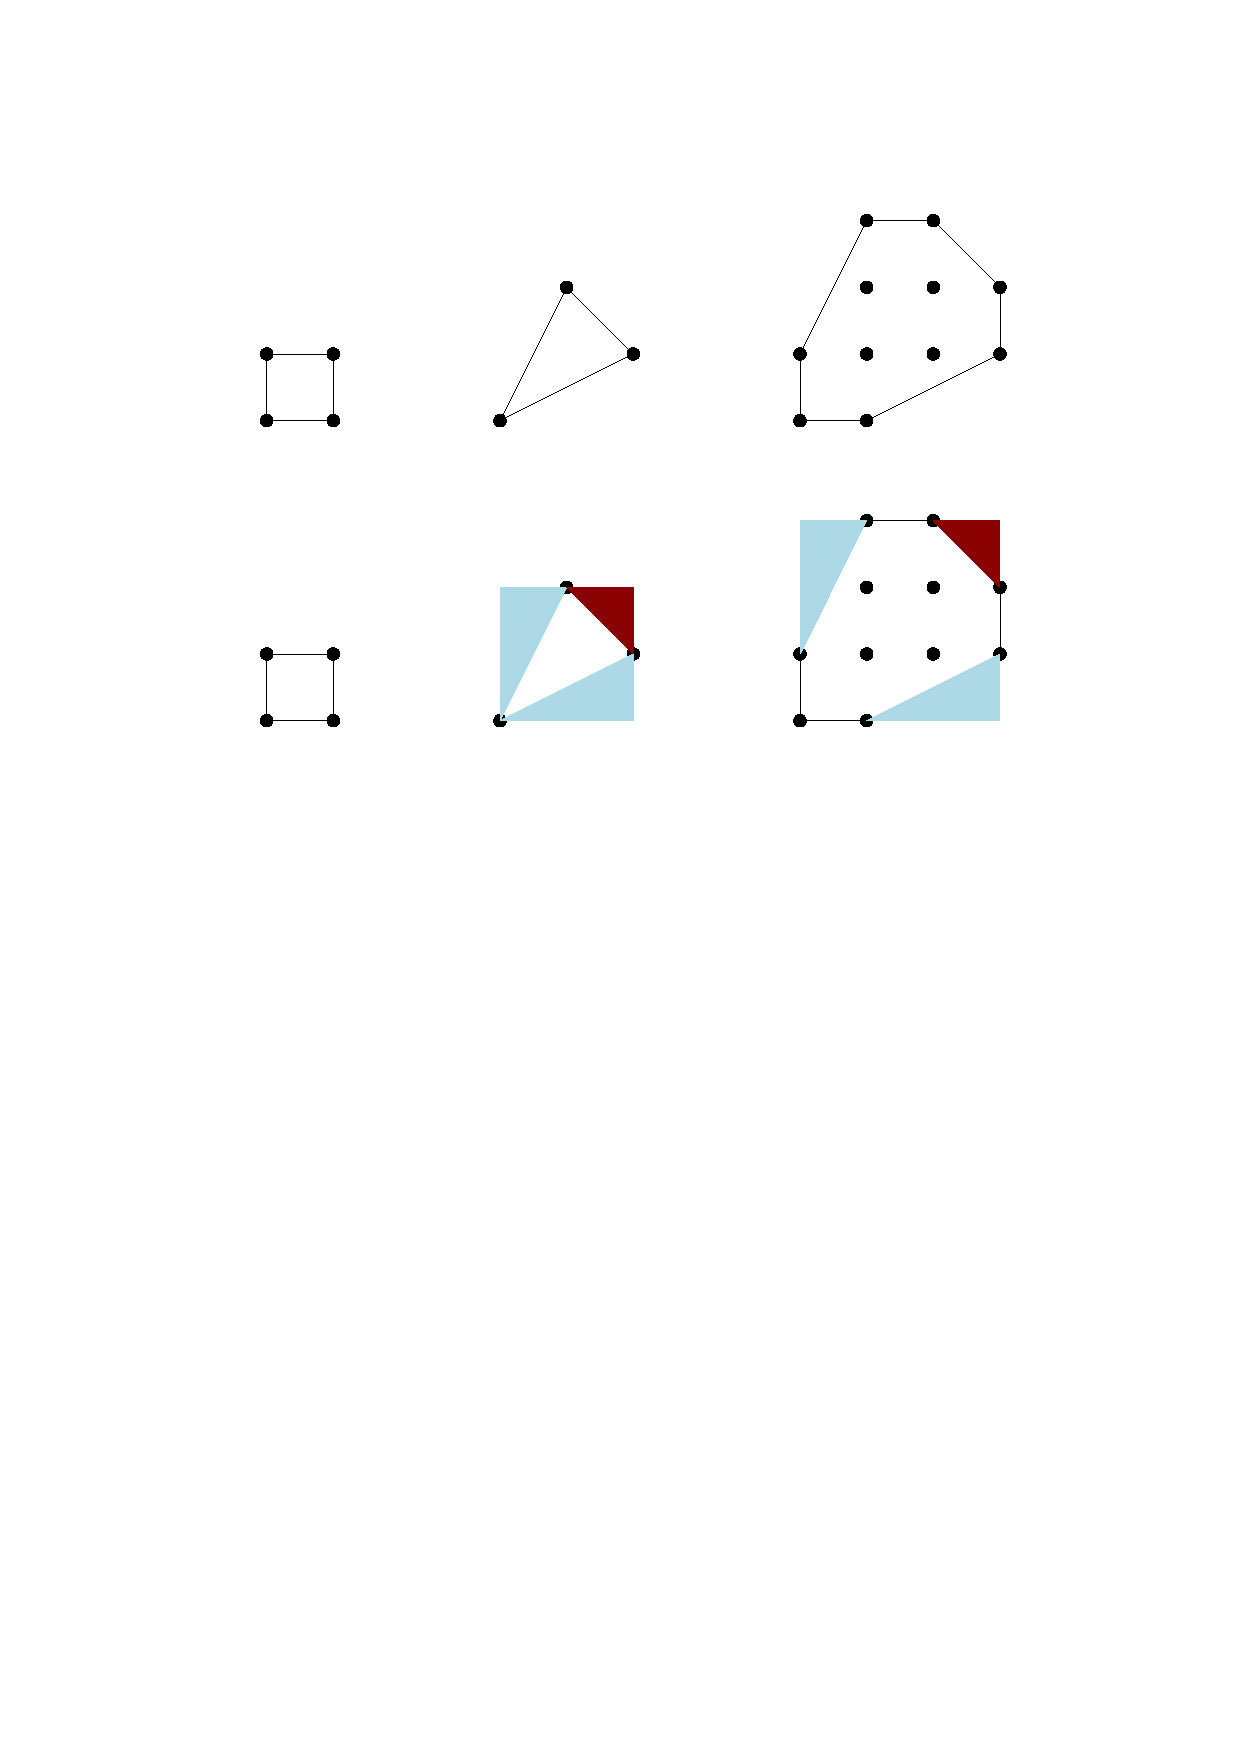
\includegraphics{Images/ConvexLattice.pdf} % requires the graphicx package
   \caption{From left to right: $P$, $Q$ and $P+Q$. The second row is with added triangles to make the calculation of the area easier.}
   \label{fig:cl}
\end{figure}
\section{d}

\section{e}
Suppose we have two lattice polygons $P$ and $Q$. Construct a polynomial $f$ as follows: starting with $f=0$, for every vertex $p_{i} = (a_{i1},a_{i2})$ of $P$ add a term to $f$ of the from $x^{a_{i1}}y^{a_{i2}}$. In this way, New($f) = P$. Analogous, construct a $g$ so that New($g)=Q$. Note that this construction is fine, since $a_{ij}$ are integers because $P,Q$ are lattices polygons. Because $P$ and $Q$ are polygons, we only have two dimensions and can use Bernstein's Theorem.\\
Using Bernstein's Theorem we find that M(New($f$),New($g)) = M(P,Q)= $ (number of solutions of the system $f(x,y)=0,g(x,y)=0$), which is an integer. 

\section{f}
Suppose we have two general plane algebraic curves $f$ and $g$ of degree $d$ and $e$ and with Newton-polygons $P=$New($f), Q=$New($g$). For the algebraic plane curve $f$ of degree $d$, we know that it is of the form $\sum_{i=0}^{d}a_{i}*x^{i}*y^{d-i}$ with all $a_{i}\neq 0$. So that the $P=$conv$(\{(i,d-i)| i\in [0,\ldots,d]\}$ which is the triangle through $(0,0),(d,0),(0,d)$. Analogous we find $Q=\Delta\{(0,0),(e,0),(0,e)\}$.\\

Now we will look at $P+Q$. When calculating $P+Q$ we should only consider the boundaries of $P$ and $Q$. From the geometric structure (both lie in the corner of the first quadrant) we see that only the hypotenusa of the triangle will be important to define $P+Q$. The points on the hypotenusa of $P$ are $\{(i,d-i)| 0\leq i\leq d, i\in \mathbb{R}\}$ and for $Q: \{(j,e-j)| 0\leq j\leq e in \mathbb{R}\}$. So the points for $P+Q$ will be $\{(i+j,e+d-i-j) | 0\leq i\leq d, 0\leq j \leq e, i,j\in \mathbb{R}\} = \{(k,e+d-k) | 0\leq k\leq d+e, k\in \mathbb{R}\}$. So we find that $P+Q$ is a right triangle with two legs of length $d+e$. 

We find: 
\[M(P,Q)= \frac{(d+e)^{2}}{2} - \frac{d^{2}}{2} -\frac{e^{2}}{2}= \frac{d^{2} + 2de + e^{2}-d^{2}-e^{2}}{2}=de\]


Consider now the functions $f$ and $g$ we used in part $c)$. We calculated $M($New($f$),New($g)=4$. From Bernstein's theorem we can find that they meet in $4$ points. We notice that $f$ and $g$ are not general polynomials, but we notice that the points defining New($f$) are contained in the Newton polynomial generated by a general polynomial of degree equal to the maximum degree of $f$. Analogous for $G$. As such, Bezout's theorem gives an upperbound for the number of meeting points, based on their degree. Here deg($f$)*deg($g)=2*3=6$ and $4\leq 6$.


\end{document}
